% -*- latex -*-
%%%%%%%%%%%%%%%%%%%%%%%%%%%%%%%%%%%%%%%%%%%%%%%%%%%%%%%%%%%%%%%%
%%%%%%%%%%%%%%%%%%%%%%%%%%%%%%%%%%%%%%%%%%%%%%%%%%%%%%%%%%%%%%%%
%%%%
%%%% This text file is part of the source of 
%%%% `Parallel Programming in MPI and OpenMP'
%%%% by Victor Eijkhout, copyright 2012-2021
%%%%
%%%% omp-examples.tex : non-trivial example programs
%%%%
%%%%%%%%%%%%%%%%%%%%%%%%%%%%%%%%%%%%%%%%%%%%%%%%%%%%%%%%%%%%%%%%
%%%%%%%%%%%%%%%%%%%%%%%%%%%%%%%%%%%%%%%%%%%%%%%%%%%%%%%%%%%%%%%%

\Level 0 {N-body problems}

So-called \indexterm{N-body problem}s come up with
we describe the interactions between a,
probably large,
number of entities under a force such as gravity.
Examples are molecular dynamics and star clusters.

While clever algorithms exist that take into account the
decay of the force over distance,
we here consider the naive algorithm that
explicitly computes all interactions.

A particle has $x,y$ coordinates and a mass~$c$.
For two particles $(x_1,y_1,c_1)$, $(x_2,y_2,c_2)$
the force on particle~1 from particle~2 is:
\[ \overrightarrow F_{12} = \frac{c_1\cdot c_2}{\sqrt{ (x_2-x_1)^2+(y_2-y_1)^2 }} \cdot \overrightarrow r_{12} \]
where $\overrightarrow r_{12}$ is the unit vector pointing from particle 2 to~1.
With $n$ particles, each particle~$i$ feels a force
\[ \overrightarrow F_i = \sum_{j\not=i} \overrightarrow F_{ij}.\]

Let's start with a couple of building blocks.
\cverbatimsnippet{ompmolaux}
Force accumulation:
\begin{lstlisting}
void add_force( struct force *f,struct force g ) {
  f->x += g.x; f->y += g.y; f->f += g.f;
}
void sub_force( struct force *f,struct force g ) {
  f->x -= g.x; f->y -= g.y; f->f += g.f;
}
\end{lstlisting}

For reference, this is the sequential code:
\cverbatimsnippet{ompmolplain}
Here $\overrightarrow F_{ij}$ is only computed for $j>i$, and then
added to both $\overrightarrow F_i$ and~$\overrightarrow F_j$.

\begin{exercise}
  Argue that both the outer loop and the inner are not directly parallelizable.
\end{exercise}

We will now explore a number of different strategies for parallelization.
All tests are done on the \indextermbus{TACC}{Frontera} cluster,
which has dual-socket \indextermbus{Intel}{Cascade Lake} nodes,
with a total of 56 cores.
Our code uses 10 thousand particles, and each interaction evaluation
is repeated 10 times to eliminate cache loading effects.

\Level 1 {Solution 1: no conflicting writes}

In our first attempt at an efficient parallel code,
we compute the full $N^2$ interactions.
One solution would be to compute the $\overrightarrow F_{ij}$
interactions for all~$i,j$,
so that there are no conflicting writes.

\cverbatimsnippet{ompmoljpar}

This increases the scalar work by a factor of two,
but surprisingly, on a single thread the run time improves:
we measure a speedup of \n{6.51} over the supposedly `optimal' code.

\begin{exercise}
  What would be an explanation?
\end{exercise}

\begin{figure}[t]
  \tikzsetnextfilename{omp-nbody1}
  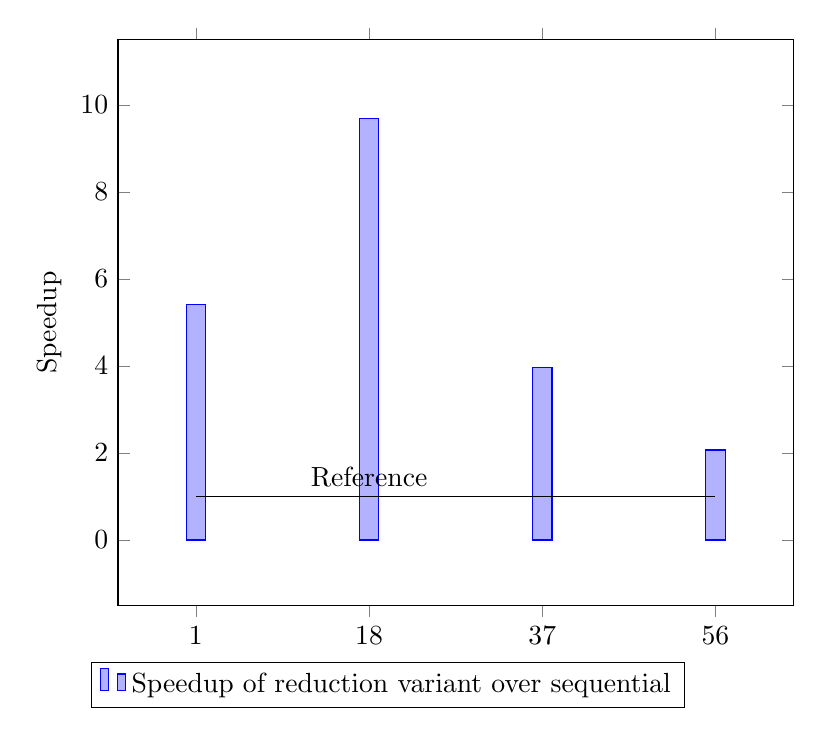
\begin{tikzpicture}  
    \begin{axis}
      [  
        ybar=3pt, bar width=7pt,
        enlargelimits=0.15,
        legend style={at={(0.4,-0.1)},anchor=north,legend columns=-1}, 
        %xlabel={\#Threads},
        ylabel={Speedup},
        symbolic x coords={1,18,37,56},
        xtick=data, ymin=0, ymax=10,
        %nodes near coords,  
        %nodes near coords align={vertical},  
      ]  
      \addplot coordinates { (1, 5.42) (18, 9.69) (37, 3.97) (56, 2.07) };
      \addplot [black,sharp plot,update limits=false]
      coordinates {(1, 1) (56, 1)}
      node[above] at (axis cs:18,1) {Reference};
      \legend{Speedup of reduction variant over sequential}
    \end{axis}
  \end{tikzpicture}  
  \caption{{Speedup of reduction variant over sequential}}
  \label{fig:omp-nbody1}
\end{figure}

However, increasing the number of threads has limited benefits for this strategy.
Figure~\ref{fig:omp-nbody1} shows that
the speedup is not only sublinear:
it actually decreases with increasing core count.

\begin{comment}
\begin{verbatim}
================ #threads = 1 ================
               Sequential: 2.029093e+01; 
       Full loop Parallel: 3.118345e+00; speedup= 6.51
================ #threads = 18 ================
       Full loop Parallel: 1.940827e+00; speedup=10.46
================ #threads = 37 ================
       Full loop Parallel: 4.390490e+00; speedup= 4.63
================ #threads = 56 ================
       Full loop Parallel: 8.484191e+00; speedup= 2.40
\end{verbatim}
\end{comment}

\begin{exercise}
  What would be an explanation?
\end{exercise}

\Level 1 {Solution 2: using atomics}

Next we try to parallelize the outer loop.
\cverbatimsnippet{ompmolipar}
To deal with the conflicting \lstinline{jp} writes,
we make the writes atomic:
\begin{lstlisting}
void sub_force( struct force *f,struct force g ) {
#pragma omp atomic
  f->x -= g.x;
#pragma omp atomic
  f->y -= g.y;
#pragma omp atomic
  f->f += g.f;
}
\end{lstlisting}

\begin{figure}[t]
  \tikzsetnextfilename{omp-nbody2}
  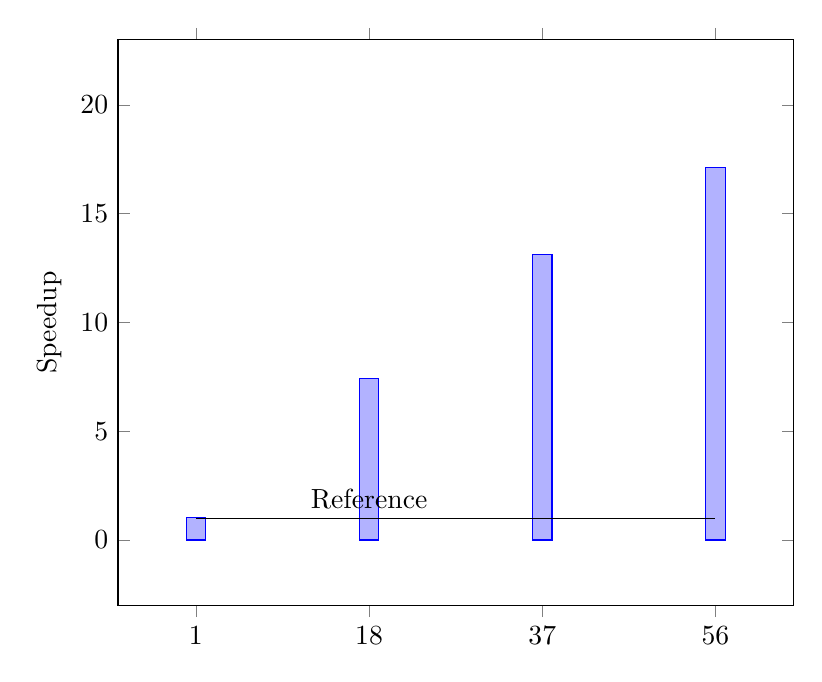
\begin{tikzpicture}  
    \begin{axis}
      [  
        ybar=3pt, bar width=7pt,
        enlargelimits=0.15,
        legend style={at={(0.4,-0.1)},anchor=north,legend columns=-1},     
        %xlabel={\#Threads},
        ylabel={Speedup},
        symbolic x coords={1,18,37,56},
        xtick=data, ymin=0, ymax=20,
        %nodes near coords,  
        %nodes near coords align={vertical},  
      ]  
      \addplot coordinates { (1, 1.02) (18, 7.43) (37, 13.11) (56, 17.11) };
      \addplot [black,sharp plot,update limits=false]
      coordinates {(1, 1) (56, 1)}
      node[above] at (axis cs:18,1) {Reference};
    \end{axis}
  \end{tikzpicture}  
  \label{fig:omp-nbody2}
  \caption{Speedup of triangular loop with atomic update}
\end{figure}

This works fairly well, as figure~\ref{fig:omp-nbody2} shows.

\begin{comment}
\begin{verbatim}
================ #threads = 1 ================
               Sequential: 2.029093e+01; 
 Triangular update atomic: 1.990096e+01; speedup= 1.02
================ #threads = 18 ================
 Triangular update atomic: 2.730043e+00; speedup= 7.43
================ #threads = 37 ================
 Triangular update atomic: 1.549876e+00; speedup=13.11
================ #threads = 56 ================
 Triangular update atomic: 1.187892e+00; speedup=17.11  
\end{verbatim}
\end{comment}

\Level 1 {Solution 3: all interactions atomic}

But if we decide to use atomic updates,
we can take the full square loop,
collapse the two loops,
and make every write atomic.
\cverbatimsnippet{ompmolijpar}

\begin{figure}[t]
  \tikzsetnextfilename{omp-nbody3}
  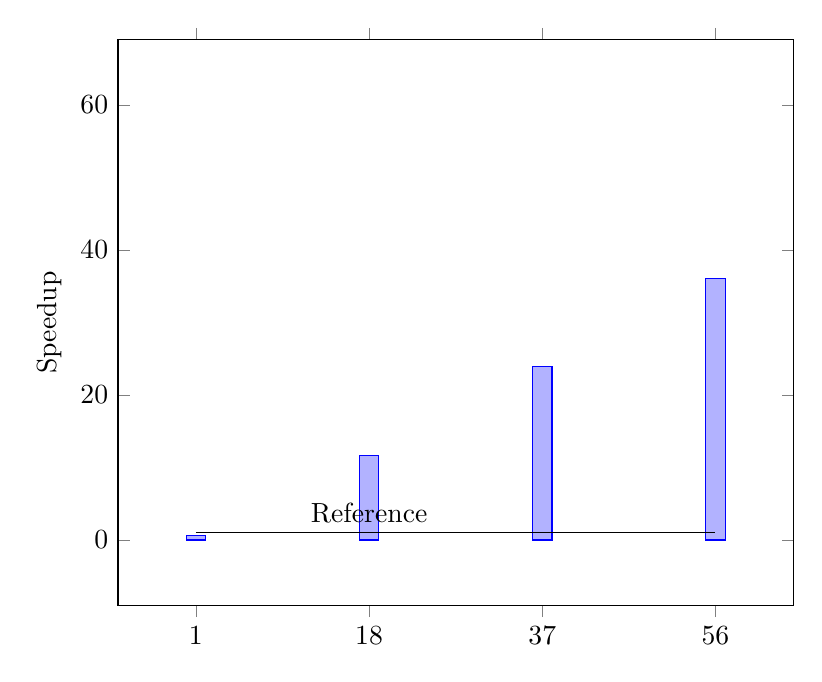
\begin{tikzpicture}  
    \begin{axis}
      [  
        ybar=3pt, bar width=7pt,
        enlargelimits=0.15,
        legend style={at={(0.4,-0.1)},anchor=north,legend columns=-1}, 
        %xlabel={\#Threads},
        ylabel={Speedup},
        symbolic x coords={1,18,37,56},
        xtick=data, ymin=0, ymax=60
        %nodes near coords,  
        %nodes near coords align={vertical},  
      ]  
      \addplot coordinates { (1, 0.65) (18, 11.7) (37, 23.9) (56, 36.1) };
      \addplot [black,sharp plot,update limits=false]
      coordinates {(1, 1) (56, 1)}
      node[above] at (axis cs:18,1) {Reference};
      %\legend{Speedup of atomic full interaction calculation}
    \end{axis}
  \end{tikzpicture}  
  \caption{Speedup of atomic full interaction calculation}
  \label{fig:omp-nbody3}
\end{figure}

Figure~\ref{fig:omp-nbody3} shows that this is pretty close to perfect.

\begin{comment}
\begin{verbatim}
================ #threads = 1 ================
               Sequential: 2.029093e+01; 
         Full loop atomic: 3.114875e+01; speedup= 0.65
================ #threads = 18 ================
         Full loop atomic: 1.739044e+00; speedup=11.67
================ #threads = 37 ================
         Full loop atomic: 8.486451e-01; speedup=23.95
================ #threads = 56 ================
         Full loop atomic: 5.630970e-01; speedup=36.09
\end{verbatim}
\end{comment}

Everything in one plot in figure~\ref{fig:omp-nbody4}.

\begin{figure}[t]
  \tikzsetnextfilename{omp-nbody4}
  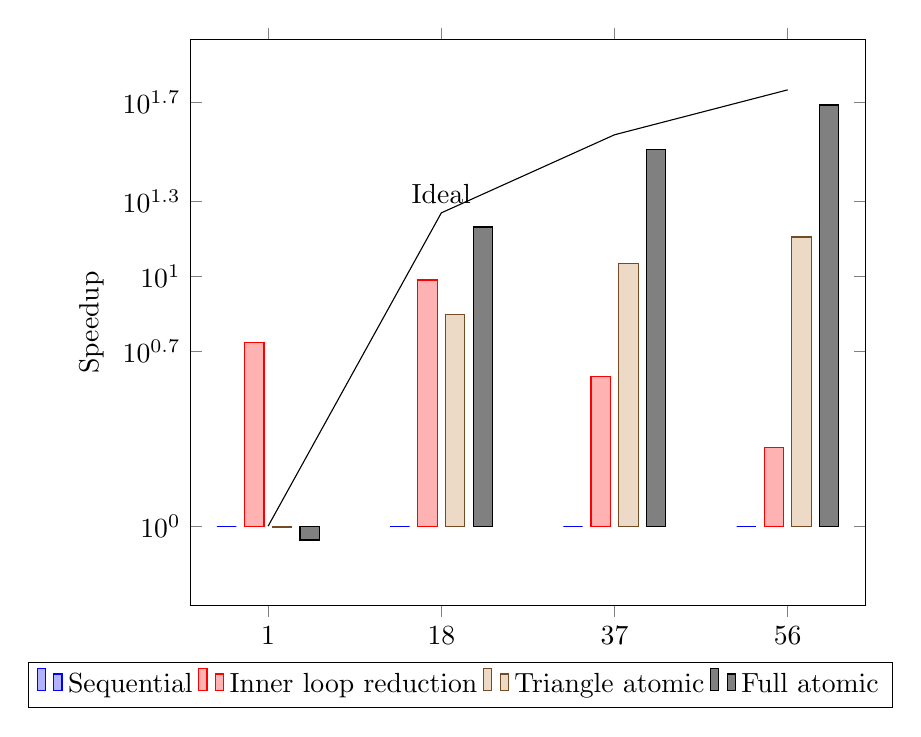
\begin{tikzpicture}  
    \begin{semilogyaxis}
      [  
        ybar=3pt, bar width=7pt,
        enlargelimits=0.15,
        legend style={at={(0.4,-0.1)},anchor=north,legend columns=-1},     
        xlabel={\#Threads},
        ylabel={Speedup},
        symbolic x coords={1,18,37,56},
        xtick=data,  ytick={1,5,10,20,50},
        %nodes near coords,  
        %nodes near coords align={vertical},  
      ]  
      \addplot coordinates {(1, 1.00) (18, 1.00) (37, 1.00) (56, 1.00)};
      \addplot coordinates {(1, 5.42) (18, 9.69) (37, 3.97) (56, 2.07)};  
      \addplot coordinates {(1, 0.99) (18, 7.02) (37, 11.3) (56, 14.4)};  
      \addplot coordinates {(1, 0.88) (18, 15.8) (37, 32.3) (56, 48.7)};  
      \addplot [black,sharp plot,update limits=false]
      coordinates {(1, 1) (18, 18) (37, 37) (56, 56)}
      node[above] at (axis cs:18,18) {Ideal};
      \legend{Sequential, Inner loop reduction, Triangle atomic, Full atomic}  
    \end{semilogyaxis}
  \end{tikzpicture}  
  \caption{All strategies together}
  \label{fig:omp-nbody4}
\end{figure}

\Level 0 {Tree traversal}

OpenMP tasks are a great way of handling trees.

In \emph{post-order tree traversal}\index{tree!traversal!post-order}
you visit the subtrees before visiting the root. This is the traversal
that you use to find summary information about a tree, for instance
the sum of all nodes, and the sums of nodes of all subtrees:

\begin{displayalgorithm}
  \For{all children $c$}
      {compute the sum $s_c$}\;
      $ s \leftarrow \sum_c s_c$
\end{displayalgorithm}

Another example is matrix factorization:
\[ S = A_{33} - A_{31}A_{11}\inv A_{13} - A_{32}A_{22}\inv A_{23} \]
where the two inverses $A_{11}\inv,A_{22}\inv$ can be computed
indepedently and recursively.

%\Level 2 {Pre-order traversal}

\begin{comment}
  https://en.wikipedia.org/wiki/Huffman_coding
\end{comment}

\Level 0 {Depth-first search}
\label{sec:omp-dfs-example}
\lstset{language=C++}

\begin{wrapfigure}{r}{3in}
  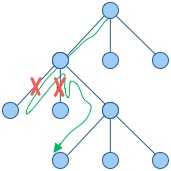
\includegraphics[scale=.7]{DFS}
\end{wrapfigure}
%
In this section we look at the `eight queens' problem, as an example of \indexac{DFS}:
is it possible to put eight queens on a chess board so that none of them threaten each other?
With \ac{DFS}, the search space of possibilities is organized as a tree
--~each partial solution leads to several possibilities for the next steps~--
which is traversed in a particular manner:
a~chain of possibilities is extended as far as feasible,
after which the search backtracks to the next chain.

The sequential implementation is easy enough.
The main program fires off:
\begin{lstlisting}
placement initial; initial.fill(empty);
auto solution = place_queen(0,initial);
\end{lstlisting}
where I hope you can take the details on trust.

The recursive call then has this structure:
\begin{lstlisting}
optional<placement> place_queen(int iqueen,const placement& current) {
  for (int col=0; col<N; col++) {
    placement next = current;
    next.at(iqueen) = col;
    if (feasible(next)) {
      if (iqueen==N-1)
	return next;
      auto attempt = place_queen(iqueen+1,next);
      if (attempt.has_value())
	return attempt;
    } // end if(feasible)
  }
  return {};
};
\end{lstlisting}
(This uses the C++17 \lstinline{optional} header.)
At each \lstinline{iqueen} level we
\begin{itemize}
\item go through a loop of all column positions;
\item filter out positions that are not feasible;
\item report success if this was the last level; or
\item recursively continue the next level otherwise.
\end{itemize}

This problem seems a prime candidate for OpenMP tasks, so we start with the usual
idiom for the main program:
%
\cxxverbatimsnippet{queensmain}

We create a task for each column, and since they are in a loop
we use \indexpragma{taskgroup} rather than \indexpragma{taskwait}.
\begin{lstlisting}
#pragma omp taskgroup
  for (int col=0; col<N; col++) {
    placement next = current;
    next.at(iqueen) = col;
#pragma omp task firstprivate(next)
    if (feasible(next)) {
    // stuff
    } // end if(feasible)
  }
\end{lstlisting}

However, the sequential program had \lstinline{return} and \lstinline{break}
statements in the loop, which is not allowed in workshare constructs
such as \indexpragma{taskgroup}.
Therefore we introduce a return variable, declared as shared:
%
\cxxverbatimsnippet{queensbreadth}

So that was easy, this computes the right solution, and it uses OpenMP tasks.
Done?

% Intel
% queens2 w/o: 10 - 0.075 - 34815, 12 - 2.54 - 841989, 13 - 17.6
%         with 10 0 0.005 - 102,   12 - 0.006 - 261,   13 - 0.006 - 111
% gcc:
%         w/o  10 - 0.080 - 34815, 12- 23.5 - 841989,  
%         with 12 - 22.9, 13 - 13.5 - 4524198

% intel
% queens0 10 - 0.032, 12 - .673, 13 - 3.8, 14 - 23.8
% gcc:
%         10 - 0.736, 12 - 22.9, 13 - 107

% seq
%         10 - 0.0001 - 102, 12 -0.0004 - 261, 13 - 0.0002 - 111, 14 - 0.0005 - 1899

\begin{figure}[ht]
  \pgfplotsset{width=4in,compat=1.7}
  \hbox\bgroup %pyskip
  \tikzsetnextfilename{omp-dfs-intel}
  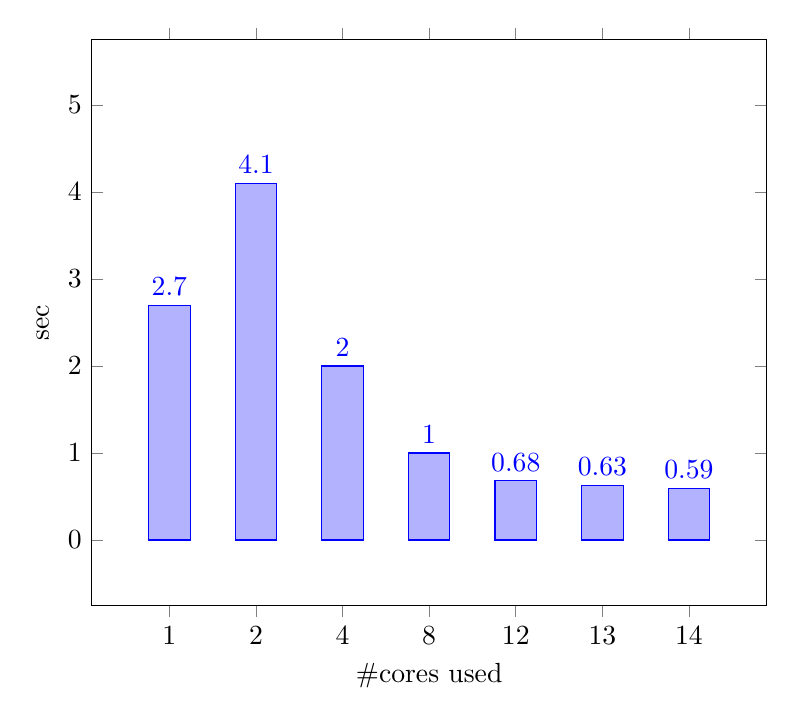
\begin{tikzpicture}  
    \begin{axis}
      [  
        ybar=3pt, bar width=15pt, enlargelimits=0.15,
        xlabel={\#cores used},
        ylabel={sec}, ymin=0.00, ymax=5,
        symbolic x coords={1,2,4,8,12,13,14},
        xtick=data,  %ytick={0,5,10,15,20,25},
        nodes near coords,  
        nodes near coords align={vertical},  
      ]  
      \addplot coordinates {(1,2.7) (2,4.1) (4,2.0) (8,1.0) (12,0.68) (13,0.63) (14,0.59) };
    \end{axis}
  \end{tikzpicture}  
  \tikzsetnextfilename{omp-dfs-gcc}
  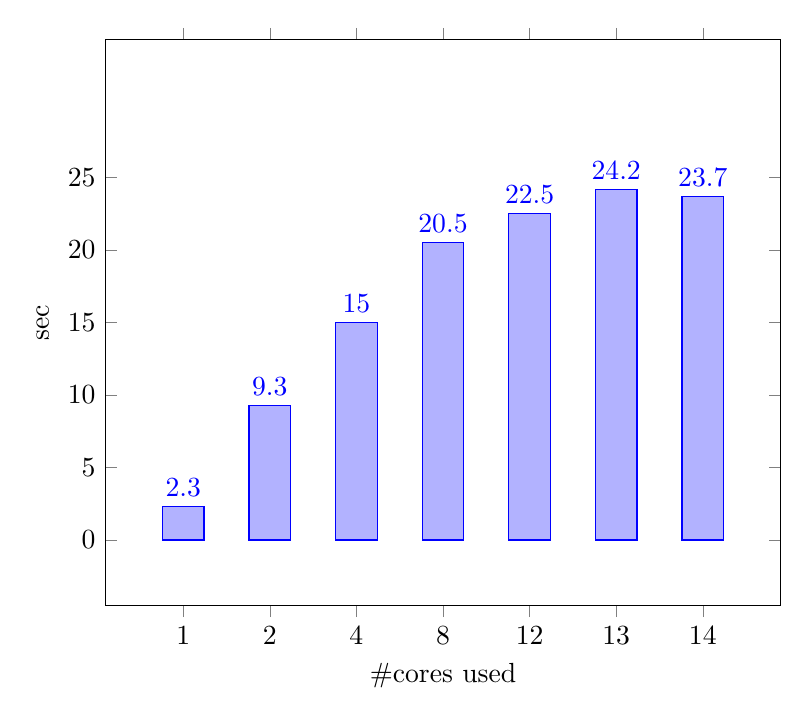
\begin{tikzpicture}  
    \begin{axis}
      [  
        ybar=3pt, bar width=15pt, enlargelimits=0.15,
        xlabel={\#cores used},
        ylabel={sec}, ymin=0.00, ymax=30,
        symbolic x coords={1,2,4,8,12,13,14},
        xtick=data,  ytick={0,5,10,15,20,25},
        nodes near coords,  
        nodes near coords align={vertical},  
      ]
      \addplot coordinates {(1,2.3) (2,9.3) (4,15.0) (8,20.5) (12,22.5) (13,24.2) (14,23.7) };
    \end{axis}
  \end{tikzpicture}  
  \egroup  %pyskip
  \caption{Using taskgroups for $N=12$; left Intel compiler, right GCC}
  \label{fig:omp-dfs}
\end{figure}

Actually this runs very slowly because,
now that we've dispensed with all early breaks from the loop,
we in effect traverse the whole search tree.
(It's not quite breadth-first, though.)
%
Figure~\ref{fig:omp-dfs} shows this for $N=12$
with the Intel compiler (version 2019) in the left panel,
and the GNU compiler (version~9.1) in the middle.
In both cases,  the blue bars give the result for the code
with only the \indexpragma{taskgroup} directive,
with time plotted as function of core count.

We see that, for the Intel compiler, running time indeed
goes down with core count.
So, while we compute too much (the whole search space),
at least parallelization helps.
With a number of threads greater than the problem size,
the benefit of parallelization disappears,
which makes some sort of sense.

We also see that the GCC compiler is really bad at OpenMP tasks:
the running time actually increases with the number of threads.

Fortunately, with \ompstandard{4} we can break out of the loop
with a \indexpragma{cancel} of the task group:
%
\cxxverbatimsnippet{queenscancel}

Surprisingly, this does not immediately give a performance improvement.
The reason for this is that cancellation is disabled by default,
and we have to set the environment variable
\begin{verbatim}
OMP_CANCELLATION=true
\end{verbatim}

\begin{figure}
  \tikzsetnextfilename{omp-dfs-cancel}
  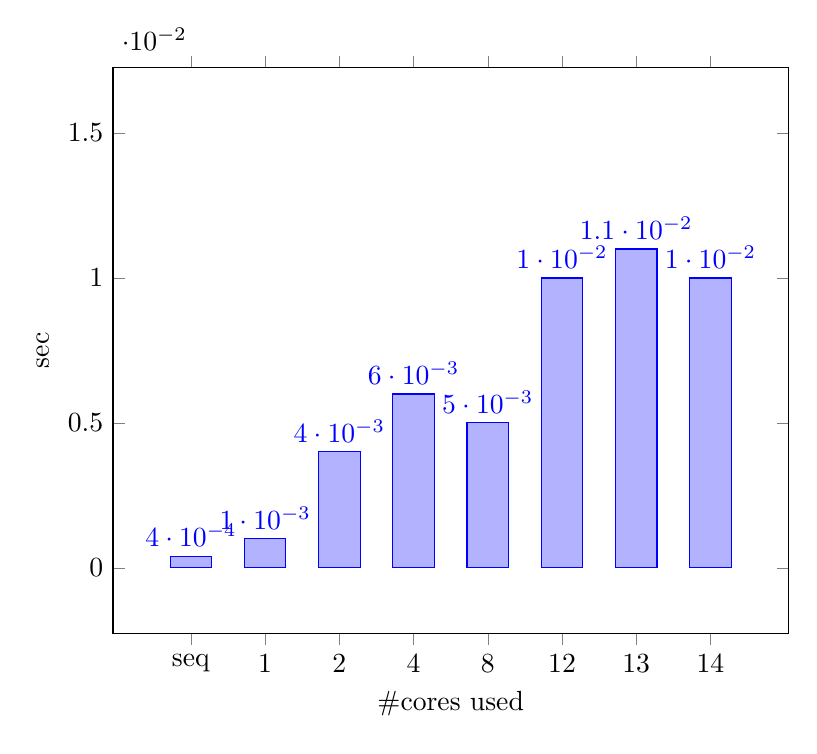
\begin{tikzpicture}  
    \begin{axis}
      [  
        ybar=3pt, bar width=15pt, enlargelimits=0.15,
        xlabel={\#cores used},
        ylabel={sec}, ymin=0.00, ymax=0.015,
        symbolic x coords={seq,1,2,4,8,12,13,14},
        xtick=data,  %ytick={0,5,10,15,20,25},
        nodes near coords,  
        nodes near coords align={vertical},  
      ]  
      \addplot coordinates {(seq,0.0004) (1,.001) (2,.004) (4,.006) (8,.005) (12,.01) (13,0.011) (14,0.010) };
    \end{axis}
  \end{tikzpicture}  
  \caption{Using taskgroup cancelling, Intel compiler}
  \label{fig:omp-dfs-cancel}
\end{figure}

With that, we get very good performance,
as  figure~\ref{fig:omp-dfs-cancel} shows,
which lists sequential time, and
multicore running time on the code with \indexpragma{cancel} directives.
Running time is now approximately the same as the sequential time.
Some questions are still left:
\begin{itemize}
\item Why does the time go up with core count?
\item Why is the multicore code slower than the sequential code,
  and would the parallel code be faster than sequential if the
  amount of scalar work (for instance in the \lstinline{feasible} function)
  would be larger?
\end{itemize}

One observation not reported here
is that the GNU compiler has basically the same running time with and without cancellation.
This is again shows that the GNU compiler is really bad at OpenMP tasks.

% Intel queens0 N=12
% make clean queens0 EXTRA_OPTIONS=-DN=12 && for t in 1 2 4 8 12 13 14 ; do  OMP_NUM_THREADS=$t ./queens0 ; done
%% computed in 2.754 seconds on 1 threads
%% computed in 4.078 seconds on 2 threads
%% computed in 2.039 seconds on 4 threads
%% computed in 1.028 seconds on 8 threads
%% computed in 0.683 seconds on 12 threads
%% computed in 0.633 seconds on 13 threads
%% computed in 0.594 seconds on 14 threads

% GCC queens0 N=12
%% computed in 2.287 seconds on 1 threads
%% computed in 9.251 seconds on 2 threads
%% computed in 15.004 seconds on 4 threads
%% computed in 20.572 seconds on 8 threads
%% computed in 22.472 seconds on 12 threads
%% computed in 24.234 seconds on 13 threads
%% computed in 23.766 seconds on 14 threads

%% Intel queens2:
%% make clean queens2 EXTRA_OPTIONS=-DN=12 && for t in 1 2 4 8 12 13 14 ; do  OMP_NUM_THREADS=$t ./queens2 ; done | grep computed
%% icpc -c queens2.cxx  -std=c++17 -qopenmp  -O2 -g -DN=12
%% icpc -o queens2 queens2.o -qopenmp
%% computed in 2.635 seconds on 1 threads
%% computed in 4.065 seconds on 2 threads
%% computed in 2.051 seconds on 4 threads
%% computed in 1.028 seconds on 8 threads
%% computed in 0.691 seconds on 12 threads
%% computed in 0.637 seconds on 13 threads
%% computed in 0.600 seconds on 14 threads
%% [c203-017 cxx:15] make clean queens2 EXTRA_OPTIONS=-DN=12 && for t in 1 2 4 8 12 13 14 ; do  OMP_NUM_THREADS=$t OMP_CANCELLATION=true ./queens2 ; done | grep computed
%% icpc -c queens2.cxx  -std=c++17 -qopenmp  -O2 -g -DN=12
%% icpc -o queens2 queens2.o -qopenmp
%% computed in 0.001 seconds on 1 threads
%% computed in 0.004 seconds on 2 threads
%% computed in 0.006 seconds on 4 threads
%% computed in 0.005 seconds on 8 threads
%% computed in 0.010 seconds on 12 threads
%% computed in 0.011 seconds on 13 threads
%% computed in 0.010 seconds on 14 threads

% GCC queens2:
%% [c203-017 cxx:17] make clean queens2 EXTRA_OPTIONS=-DN=12 && for t in 1 2 4 8 12 13 14 ; do  OMP_NUM_THREADS=$t ./queens2 ; done | grep computed
%% g++ -c queens2.cxx  -std=c++17 -ggdb -fopenmp -O2 -g -DN=12
%% g++ -o queens2 queens2.o -ggdb -fopenmp -lm
%% computed in 2.354 seconds on 1 threads
%% computed in 8.614 seconds on 2 threads
%% computed in 15.041 seconds on 4 threads
%% computed in 20.169 seconds on 8 threads
%% computed in 22.997 seconds on 12 threads
%% computed in 24.207 seconds on 13 threads
%% computed in 23.139 seconds on 14 threads
%% [c203-017 cxx:18] make clean queens2 EXTRA_OPTIONS=-DN=12 && for t in 1 2 4 8 12 13 14 ; do  OMP_NUM_THREADS=$t OMP_CANCELLATION=true ./queens2 ; done | grep computed
%% g++ -c queens2.cxx  -std=c++17 -ggdb -fopenmp -O2 -g -DN=12
%% g++ -o queens2 queens2.o -ggdb -fopenmp -lm
%% computed in 2.329 seconds on 1 threads
%% computed in 8.841 seconds on 2 threads
%% computed in 15.836 seconds on 4 threads
%% computed in 19.302 seconds on 8 threads
%% computed in 22.437 seconds on 12 threads
%% computed in 23.467 seconds on 13 threads
%% computed in 24.027 seconds on 14 threads


\lstset{language=C}
